\documentclass[12pt,letterpaper]{article}
\usepackage{graphicx,textcomp}
\usepackage{natbib}
\usepackage{setspace}
\usepackage{fullpage}
\usepackage{color}
\usepackage[reqno]{amsmath}
\usepackage{amsthm}
\usepackage{fancyvrb}
\usepackage{amssymb,enumerate}
\usepackage[all]{xy}
\usepackage{endnotes}
\usepackage{lscape}
\newtheorem{com}{Comment}
\usepackage{float}
\usepackage{hyperref}
\newtheorem{lem} {Lemma}
\newtheorem{prop}{Proposition}
\newtheorem{thm}{Theorem}
\newtheorem{defn}{Definition}
\newtheorem{cor}{Corollary}
\newtheorem{obs}{Observation}
\usepackage[compact]{titlesec}
\usepackage{dcolumn}
\usepackage{tikz}
\usetikzlibrary{arrows}
\usepackage{multirow}
\usepackage{xcolor}
\newcolumntype{.}{D{.}{.}{-1}}
\newcolumntype{d}[1]{D{.}{.}{#1}}
\definecolor{light-gray}{gray}{0.65}
\usepackage{url}
\usepackage{listings}
\lstset{language=R} %% Mio
\usepackage{color}

\definecolor{codegreen}{rgb}{0,0.6,0}
\definecolor{codegray}{rgb}{0.5,0.5,0.5}
\definecolor{codepurple}{rgb}{0.58,0,0.82}
\definecolor{backcolour}{rgb}{0.95,0.95,0.92}

\lstdefinestyle{mystyle}{
	backgroundcolor=\color{backcolour},   
	commentstyle=\color{codegreen},
	keywordstyle=\color{magenta},
	numberstyle=\tiny\color{codegray},
	stringstyle=\color{codepurple},
	basicstyle=\footnotesize,
	breakatwhitespace=false,         
	breaklines=true,                 
	captionpos=b,                    
	keepspaces=true,                 
	numbers=left,                    
	numbersep=5pt,                  
	showspaces=false,                
	showstringspaces=false,
	showtabs=false,                  
	tabsize=2
}
\lstset{style=mystyle}
\newcommand{\Sref}[1]{Section~\ref{#1}}
\newtheorem{hyp}{Hypothesis}

\title{Problem Set 1 - Answers}
\date{Due: October 1, 2023}
\author{Applied Stats/Quant Methods 1}

\begin{document}
	\maketitle
	
	\section*{Instructions}
	\begin{itemize}
	\item Please show your work! You may lose points by simply writing in the answer. If the problem requires you to execute commands in \texttt{R}, please include the code you used to get your answers. Please also include the \texttt{.R} file that contains your code. If you are not sure if work needs to be shown for a particular problem, please ask.
\item Your homework should be submitted electronically on GitHub.
\item This problem set is due before 23:59 on Sunday October 1, 2023. No late assignments will be accepted.
\item Total available points for this homework is 80.
	\end{itemize}
	
	\vspace{1cm}
	\section*{Question 1 (40 points): Education}

A school counselor was curious about the average of IQ of the students in her school and took a random sample of 25 students' IQ scores. The following is the data set (data set provided):\\
\vspace{.5cm}

\vspace{1cm}

\begin{enumerate}
	\item Find a 90\% confidence interval for the average student IQ in the school.\\
	
	\item Next, the school counselor was curious  whether  the average student IQ in her school is higher than the average IQ score (100) among all the schools in the country.\\ 
	
	\noindent Using the same sample, conduct the appropriate hypothesis test with $\alpha=0.05$.
\end{enumerate}

\newpage


\noindent {\Large \textbf{Answers to Question 1:}} \\

\noindent \textbf {Confidence Interval}

\begin{itemize}
	\item  First, to calculate the confidence interval, since I do not know the SD for the population, and since n = 25 (while our threshold is 30), I must do a T test, rather than a Z test. I learned from \href{https://www.statology.org/working-with-the-student-t-distribution-in-r-dt-qt-pt-rt/}{this source}  that I can thus use qt instead of qnorm.
	\item I also know that my T statistic will be =  (sample mean - pop mean) / (s/sqrt(n)) , and
	\item It will be between the following critical values:  - T(n-1, alpha/2) <= T stat <= T(n-1, alpha/2)
	\item Solving for pop mean in my T statistic, the CI will have the following lower and upper bounds:
	\item Sample mean - T(n-1, alpha/2)(s/sqrt(n)) , sample mean + T(n-1, alpha/2)(s/sqrt(n))

\end{itemize}

In R, I make all the necessary calculations, and I obtain: 

\begin{itemize}
\item mean(y) = 98.44
\item sd(y) = 13.09
\item sqrt(n) = 5
\end{itemize}

And I know that:

\begin{itemize}
\item alpha = 1 - confidence = 0.1
\item And that degrees of freedom = n -1 = 24
\end{itemize}

\noindent After inputting alpha/2 and n-1 degrees of freedom into qt, I obtain a \textbf{critical value of 1.710882}. \\

\noindent Multiplying my critical value by s/sqrt(n), I obtain  \textbf{4.480072}, which I must add and substract to the sample mean to get my upper and lower bounds. \\

\noindent This substraction and addition results in a  \textbf{CI that goes from 93.95993 to 102.92007}. \\

\noindent Finally, I confirm this result with the function t.test() and the resulting 90 percent confidence interval is identical. I also wish to see what happens if I use qnorm instead of qt in this case, and the resulting CI is slightly different. \\

\noindent \textbf{Interpretation:} Now I can tell that, if multiple samples were drawn from the same population (in this case, the entire population of students in the school) and a 95\% CI were calculated for each sample, I would expect the population mean to be found within 95% of these CIs. 


\newpage

\noindent \textbf {Relevant R Code for Confidence Interval}

\lstinputlisting[language=R, linerange={28-31, 34-58}]{PS01_SC_answers.R}

\newpage

\noindent \textbf {Hypothesis Testing} \\

\noindent Now I wish to conduct a hypothesis test to see if the school mean (the population mean) is greater than 100. \\

\noindent !! Assuming that, for the whole school, IQs are distributed normally, and that the sample was taken using randomization, and knowing that I am dealing with continuous data: 

\begin{itemize}
\item I wish to test if the school mean is greater than 100, so I set up my Null (H0) and Alternative (Ha) Hypotheses accordingly: 
\item H0:  mean school is lesser or equal to 100
\item Ha: mean school is greater than 100
\end{itemize}

I must use T test, where 
\begin{itemize}
\item alpha = 1 - Confidence = 0.05, and
\item the degrees of freedom, like with the CI, are still 24.
\end{itemize}

\noindent If T is greater than T(n = 24, alpha = 0.05), I may reject H0 at the 95 confidence level. \\
\noindent And T = (mean(y) - 100) / (sd(y)/sqrt(25))

\begin{itemize}
\item Calculating the T statistic in R, using qt, I obtain -0.5957439 
\item And my critical value is  1.710882
\item Since T is NOT greater than the critical value I may NOT reject H0 at the 95\% confidence level
\end{itemize}

Alternatively, comparing my p-value with alpha: 

\begin{itemize}
\item In R, using pt, I obtain a p-value of 0.7215383. 
\item This is much larger than my alpha = 0.05; thus I may not reject H0.
\end{itemize}

\noindent \textbf{Interpretation:} After conducting a hypothesis test at the 95\% confidence level to see if the school mean (population mean) is greater than 100, not enough evidence was found to reject the null hypothesis that the mean is smaller or equal to 100; or to support the alternative hypothesis that the mean is greater than 100. 

\newpage

\noindent \textbf {Relevant R Code for Hypothesis Testing}

\lstinputlisting[language=R, linerange={68-86}]{PS01_SC_answers.R}

\newpage

\newpage

	\section*{Question 2 (40 points): Political Economy}

\noindent Researchers are curious about what affects the amount of money communities spend on addressing homelessness. The following variables constitute our data set about social welfare expenditures in the USA. \\
\vspace{.5cm}


\begin{tabular}{r|l}
	\texttt{State} &\emph{50 states in US} \\
	\texttt{Y} & \emph{per capita expenditure on shelters/housing assistance in state}\\
	\texttt{X1} &\emph{per capita personal income in state} \\
	\texttt{X2} &  \emph{Number of residents per 100,000 that are "financially insecure" in state}\\
	\texttt{X3} &  \emph{Number of people per thousand residing in urban areas in state} \\
	\texttt{Region} &  \emph{1=Northeast, 2= North Central, 3= South, 4=West} \\
\end{tabular}

\vspace{.5cm}
\noindent Explore the \texttt{expenditure} data set and import data into \texttt{R}.
\vspace{.5cm}
\vspace{.5cm}
\begin{itemize}

\item
Please plot the relationships among \emph{Y}, \emph{X1}, \emph{X2}, and \emph{X3}? What are the correlations among them (you just need to describe the graph and the relationships among them)?
\vspace{.5cm}
\item
Please plot the relationship between \emph{Y} and \emph{Region}? On average, which region has the highest per capita expenditure on housing assistance?
\vspace{.5cm}
\item
Please plot the relationship between \emph{Y} and \emph{X1}? Describe this graph and the relationship. Reproduce the above graph including one more variable \emph{Region} and display different regions with different types of symbols and colors.
\end{itemize}

\newpage


\noindent {\Large \textbf{Answers to Question 2:}} \\

\noindent \textbf {Part 1}

\begin{itemize}

\item When plotting X1 against Y, that is per capita personal income against per capita expenditure on shelters/housing assistance, a pattern does emerge; the data are a little concentrated along a line with a positive slope, showing a positive correlation between the two variables. The association may not be very strong, as the dots are quite dispersed with some outliers, but it is nonetheless visible. 

\item When plotting X2 against Y, that is the number of residents per 100,000 who are financially insecure, against per capita expenditure on shelters/housing assistance, the two variables do not seem to be associated linearly. Rather, from looking at the plot, it could be that, before X2 = 300, the number of residents who are financially insecure is negatively associated with per capita expenditure on shelters/housing assistance, but once the 300 threshold is passed on X2, the relationship between the number of financially insecure people and expenditure seems to become positive. This association would perhaps be best represented by a quadratic equation, and there does not seem to be a linear correlation between the two. 

\item When plotting X3 against Y, that is the number of people per 1000 who reside in urban areas, against per capita expenditure on shelters/housing assistance, there seems to be a positive correlation between the two variables. The pattern that emerges suggests the data are concentrated along a line with a positive slope, with a couple of considerable outliers in the lower-right corner. 

\item When plotting X1 against X2, that is per capita personal income against the number of residents per 100,000 who are financially insecure, the two variables seem to be unrelated in the scatterplot. No obvious pattern emerges; rather, the observations are dispersed all over the area of the plot. 

\item When plotting X1 against X3, that is per capita personal income against the number of residents per 1000 who live in urban areas, the two variables seem to be positively correlated, and the dots form a pattern that could adjust to a line with positive slope. 

\item Finally, when plotting X2 against X3, that is the number of residents per 100,000 who are financially insecure against the number of people per 1000 who live in urban areas, there seems to be no relationship between the two. The scatterplot reveals that observations are disperes all over the area of the plot. 

\end{itemize}

\newpage

\noindent \textbf {Part 2}

\begin{itemize}
\item When plotting the relationship between Y and Region, that is the per capita expenditure on shelters/housing assistance by region, the graph that emerges suggests that Region 4 (the West) has the highest per capita expenditure, on average, although from the plot it is also visible that this region has the largest variance in expenditure. 
\item Also, to confirm, we may use R to group the observations in the expenditure dataset by region, and then obtain the mean for each group. This exercise shows that Region 4 has an average per capita expenditure of \$ 88.30 on shelters/housing assistance, which is higher than the mean values for the other three regions. 
\end{itemize}

\noindent \textbf {Part 3}

\begin{itemize}
\item The relationship between X1 and Y has already been described in Part 1 above, and when adding the different colors and dot shapes by region, we gain some new insights: 
\item For Regions 1 and 3, there does seem to be a positive correlation between X1 and Y, as both the red and blue dots seem to gather around lines with positive slopes. 
\item For Regions 2 and 4, however, this is a lot less clear, as the green and purple dots are dispersed around a large area of the plot, forming no evident pattern. 
\end{itemize}
 
 \newpage
 
 \noindent \textbf {Relevant R Code for Question 2 (Plotting)}
 
 \lstinputlisting[language=R, linerange={97-127,132-153}]{PS01_SC_answers.R}
 
\noindent Please note that I was not able to make the scatterplot do what I needed it to do with the colors and dot shapes per group, so I did it with ggplot. I already knew ggplot from before, but I did consult two sources to remember what exactly I needed to input to make the plot I needed. There are more details about this and these sources in my R script.

 \newpage

 \noindent \textbf {Plots that resulted from Question 2} \\
  
 
 \begin{figure}[htbp]
 \centering
 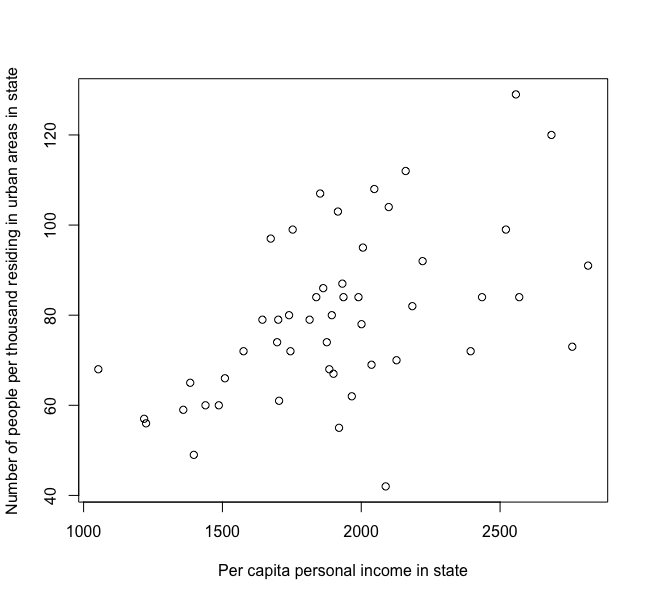
\includegraphics[width=0.8\linewidth]{/Users/sarabcidf/Desktop/ASDS/Statistics/GitRep/problemSets/PS01/my_answers/Rplot1.png}
 \caption{Plot1}
 \end{figure}
 
  \begin{figure}
 \centering
 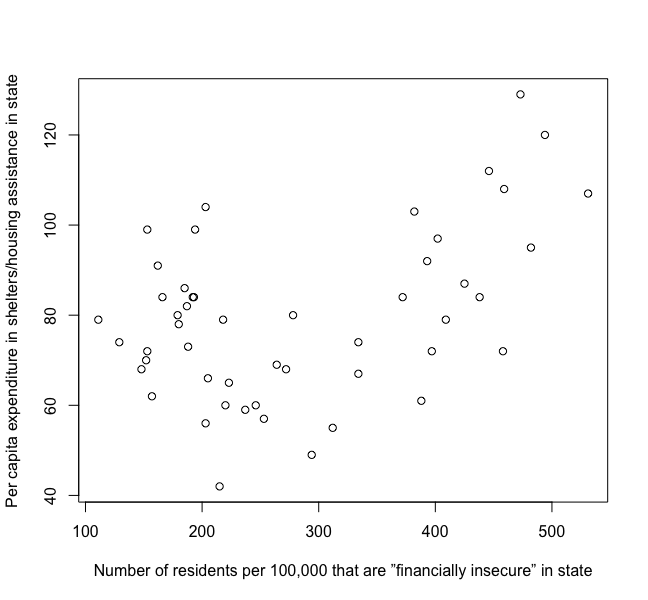
\includegraphics[width=0.8\linewidth]{/Users/sarabcidf/Desktop/ASDS/Statistics/GitRep/problemSets/PS01/my_answers/Rplot2.png}
 \caption{Plot2}
 \end{figure}
 
  \begin{figure}
 \centering
 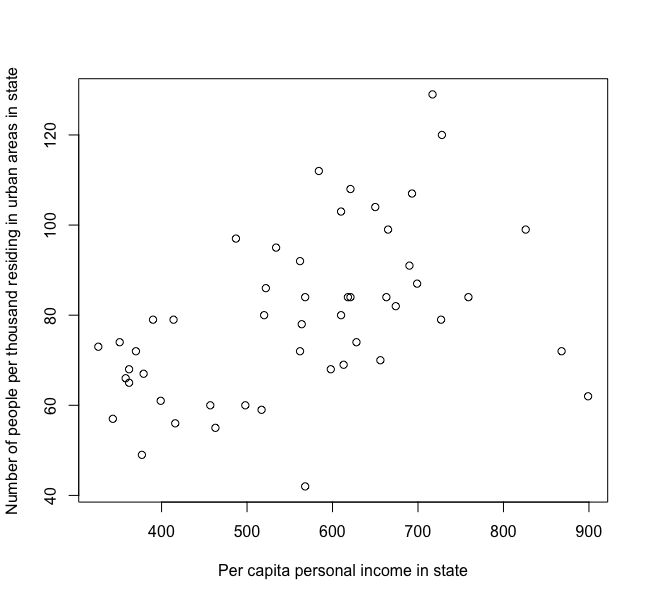
\includegraphics[width=0.8\linewidth]{/Users/sarabcidf/Desktop/ASDS/Statistics/GitRep/problemSets/PS01/my_answers/Rplot3.png}
 \caption{Plot3}
 \end{figure}
 
  \begin{figure}
 \centering
 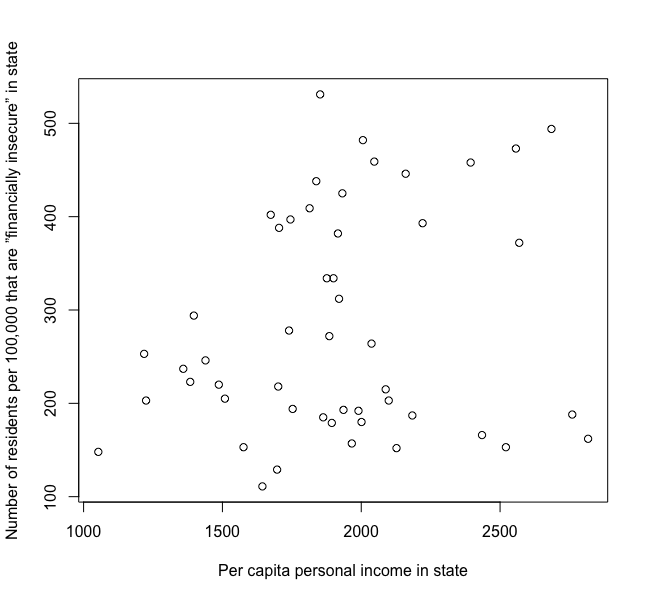
\includegraphics[width=0.8\linewidth]{/Users/sarabcidf/Desktop/ASDS/Statistics/GitRep/problemSets/PS01/my_answers/Rplot4.png}
 \caption{Plot4}
 \end{figure}
 
  \begin{figure}
 \centering
 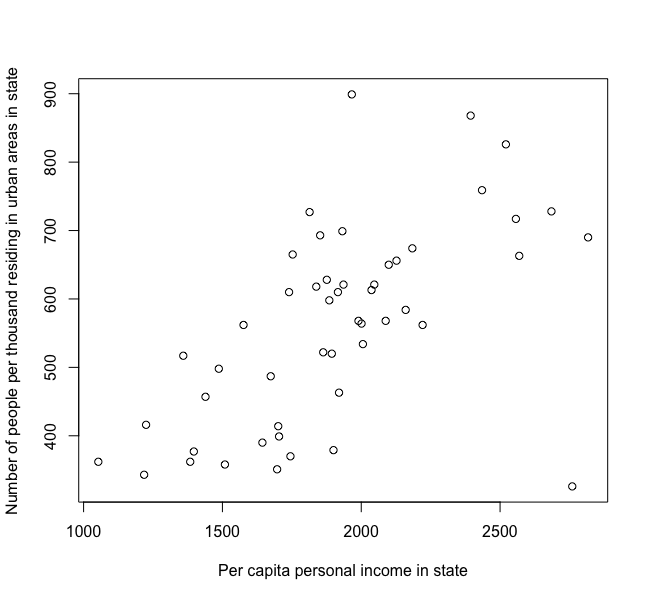
\includegraphics[width=0.8\linewidth]{/Users/sarabcidf/Desktop/ASDS/Statistics/GitRep/problemSets/PS01/my_answers/Rplot5.png}
 \caption{Plot5}
 \end{figure}
 
  \begin{figure}
 \centering
 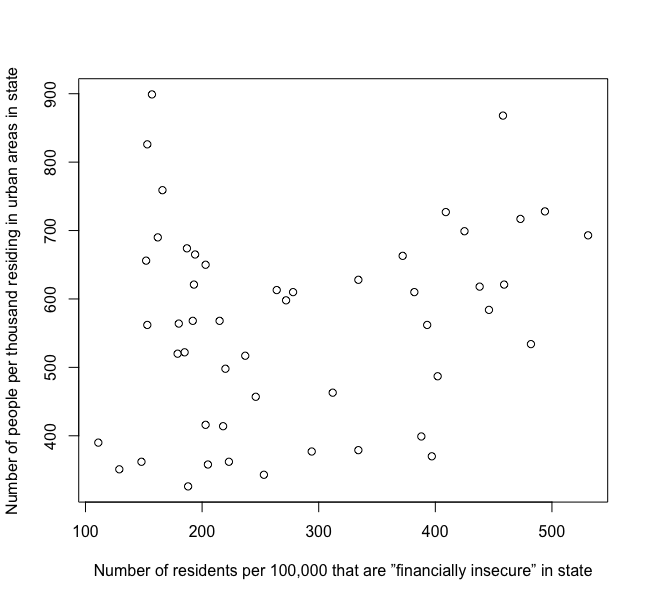
\includegraphics[width=0.8\linewidth]{/Users/sarabcidf/Desktop/ASDS/Statistics/GitRep/problemSets/PS01/my_answers/Rplot6.png}
 \caption{Plot6}
 \end{figure}
 
   \begin{figure}
 	\centering
 	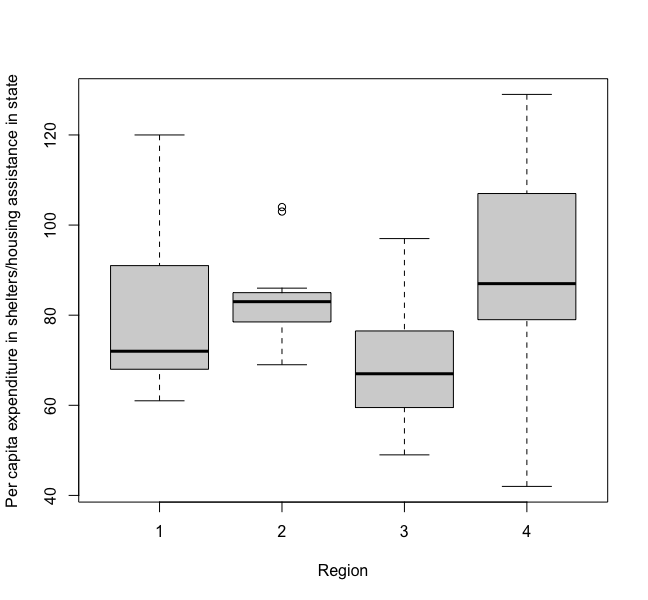
\includegraphics[width=0.8\linewidth]{/Users/sarabcidf/Desktop/ASDS/Statistics/GitRep/problemSets/PS01/my_answers/Rplot7.png}
 	\caption{Plot7}
 \end{figure}
 
  \begin{figure}
 \centering
 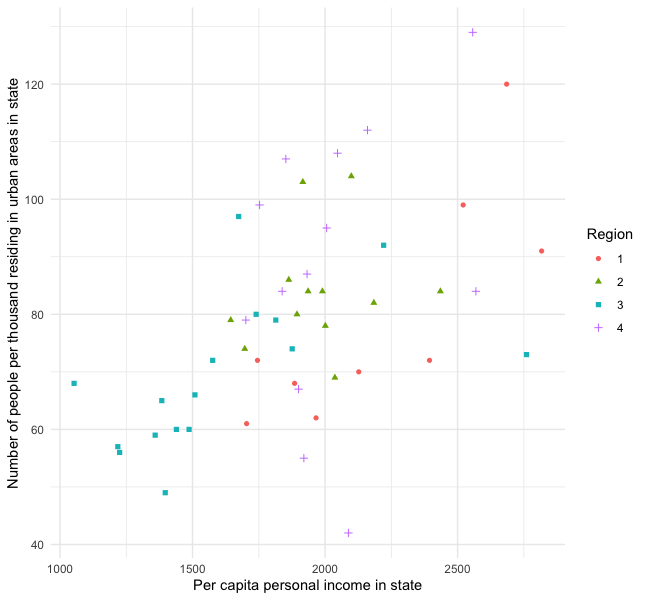
\includegraphics[width=0.8\linewidth]{/Users/sarabcidf/Desktop/ASDS/Statistics/GitRep/problemSets/PS01/my_answers/Rplot8.png}
 \caption{Plot8}
 \end{figure}
 
 \noindent Please also note that I consulted overleaf.com several times throughout this assignment to fix issues with LaTeX. For example, I learned \href{http://www.overleaf.com}{here} how to include URLs in the document. I also consulted overleaf.com because I was having trouble making the first of the plots above go where I wanted it to go; that is where I saw that including [htbp] next to "begin figure" makes it go where we mark it, since the default is something different! 

\end{document}
